\sujet{Geometry}

\noindent
Duration : 45mn - 10 points\\
{\bf Please, send your final codes to: \texttt{debayle@emse.fr}}\\


\section{Geometrical characterization}
\index{Characterization}
\index{Segmentation}

\begin{figure}[htbp]
 \centering
 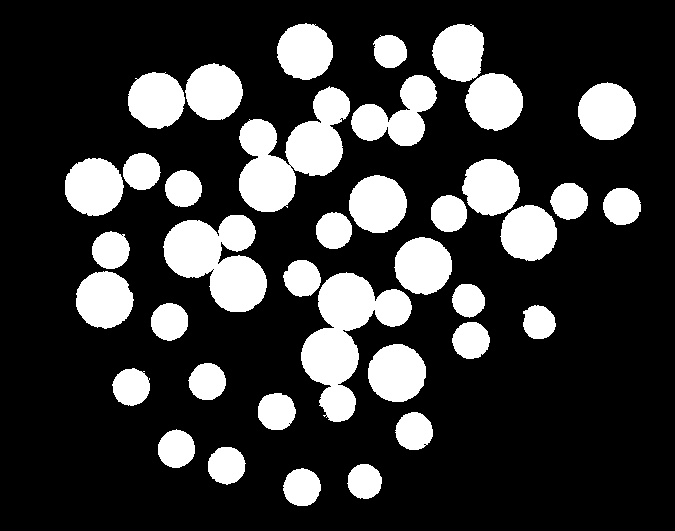
\includegraphics[width=8cm]{disks.png}
 \caption{This image contains circular particles with 2 different sizes.}
 \label{fig:exam_2016:disks}
\end{figure}

\begin{qbox}
With the image of Fig.\ref{fig:exam_2016:disks}, propose a method to automatically count the number of particles of each size (small and large).
\end{qbox}


